\documentclass{article}
\usepackage[nonatbib]{nips_2016}

\def\COMPLETE{}
\usepackage[boxruled]{algorithm2e}
\usepackage{amsmath,amssymb,amstext,amsthm}

\usepackage[utf8]{inputenc} % allow utf-8 input
\usepackage[T1]{fontenc}    % use 8-bit T1 fonts
\usepackage{hyperref}       % hyperlinks
\usepackage{url}            % simple URL typesetting
\usepackage{booktabs}       % professional-quality tables
\usepackage{amsfonts}       % blackboard math symbols
\usepackage{nicefrac}       % compact symbols for 1/2, etc.
\usepackage{microtype}      % microtypography

\usepackage{graphicx}
\usepackage{hyperref}

\usepackage{xr}
\externaldocument[A-]{figures/activeClustering}

\usepackage{color}
\usepackage[toc,page]{appendix}
\usepackage{xspace}
\usepackage[inline]{enumitem}
\usepackage{times}
\usepackage{float}
\usepackage{capt-of}

\usepackage{bbm}

\usepackage{tikz}
\usetikzlibrary{shapes, calc, arrows, through, intersections, decorations.pathreplacing, patterns}

\newcommand{\mc}{\mathcal}
\newcommand{\mb}{\mathbf}
\DeclareMathOperator*{\argmin}{arg\,min}
\DeclareMathOperator*{\argmax}{arg\,max}
\DeclareMathOperator{\vcdim}{VC-Dim}
\DeclareMathOperator{\vol}{vol}

\renewcommand\labelitemi{$\bullet$}
\renewcommand{\labelitemii}{$\star$}

\newtheorem{theorem}{Theorem}
\newtheorem{lemma}[theorem]{Lemma}
\newtheorem{definition}[theorem]{Definition}
\newtheorem{proposition}[theorem]{Proposition}
\newtheorem{corollary}[theorem]{Corollary}



\newcommand{\todo}{\textcolor{blue}{[TODO]}\xspace}
\newcommand{\complete}{\textcolor{red}{[TO BE COMPLETED]}\xspace}
\newcommand{\wip}{\textcolor{red}{[Work in progress]}\xspace}
\newcommand{\multlinecomment}[1]{\directlua{-- #1}}




\newcommand{\fix}{\textcolor{blue}{[FIX]}\xspace}
\newcommand{\q}{\textcolor{blue}{[?]}\xspace}

\title{Clustering with Same-Cluster Queries}
%\institute{School of Computer Science\\University of Waterloo\\ Waterloo, ON, N2L 3G1 \\CANADA \\ \email{\{skushagr@,shai@cs.\}uwaterloo.ca}}


%%%%% Document Body %%%%%
\begin{document}
\maketitle

\appendix
\section{Relationships Between Query Models}
\label{appendix:diffQueryModels}

\begin{proposition}
Any clustering algorithm that uses only $q$ same-cluster queries can be adjusted to use $2q$ cluster-assignment queries (and no same-cluster queries) with the same order of time complexity.
\end{proposition}
\begin{proof}
We can replace each same-cluster query with two cluster-assignment queries as in $Q(x_1,x_2)={\mathbbm{1}}\{Q(x_1)=Q(x_2))\}$.
\end{proof}

\begin{proposition}
Any algorithm that uses only $q$ cluster-assignment queries can be adjusted to use $kq$ same-cluster queries (and no cluster-assignment queries) with at most a factor $k$ increase in computational complexity, where $k$ is the number of clusters.
\end{proposition}
\begin{proof}
If the clustering algorithm has access to an instance from each of $k$ clusters (say $x_i\in X_i$), then it can simply simulate the cluster-assignment query by making $k$ same-cluster queries ($Q(x) = \argmax_{i}\mathbbm{1}\{Q(x, x_i)\}$). Otherwise, assume that at the time of querying $Q(x)$ it has only instances from $k^\prime<k$ clusters. In this case, the algorithm can do the same with the $k^\prime$ instances and if it does not find the cluster, assign $x$ to a new cluster index. This will work, because in the clustering task the output of the algorithm is a partition of the elements, and therefore the indices of the clusters do not matter.
\end{proof}


\section{Comparison of $\gamma$-Margin and $\alpha$-Center Proximity}
\label{appendix:gammaMrginVsAlphaCenter}

\begin{definition}[$\alpha$-center proximity \cite{awasthi2012center}]
\label{defn:alphacp}
Given a clustering instance $(\mc X, d)$ in some metric space $M$ and the number of clusters $k$. We say that a clustering $\mc C_{\mc X} = \{C_1, \ldots, C_k\}$ induced by centers $c_1, \ldots, c_k \in M$ has $\alpha$-center proximity w.r.t $\mc X$ and $k$ if the following holds. For all $x \in C_i$ and $i\neq j$, 
$$\alpha d(x, c_i) < d(x, c_j)$$
\end{definition}
In this paper, we introduced a notion of $\gamma$-margin. We gave upper (with query) and lower bounds on $\gamma$, when the metric space $M$ is euclidean and the centers are allowed be points in the metric space. Another notion of niceness of clusterability is $\alpha$-center proximity. This notion has been considered in the past in various works \cite{balcan2012clustering,awasthi2012center}. However, the problem setting in these works was different from our current setting. While in the current work, we were focussed on the euclidean metric space, these works considered arbitrary metric space. 

\begin{table}[]
\centering
\caption{Known results for $\alpha$-center proximity}
\label{table:alphacp}
\begin{tabular}{lll}
\cline{2-3}
\multicolumn{1}{l|}{} & \multicolumn{1}{l|}{Euclidean} & \multicolumn{1}{l|}{Non-euclidean} \\ \hline
\multicolumn{1}{|l|}{\begin{tabular}[c]{@{}l@{}}Centers \\ from data\end{tabular}} & \multicolumn{1}{l|}{?} & \multicolumn{1}{l|}{\begin{tabular}[c]{@{}l@{}}Upper bound \cite{balcan2012clustering} - $\sqrt{2}+1$\\ Lower bound \cite{ben2014data} - 2\end{tabular}} \\ \hline
\multicolumn{1}{|l|}{\begin{tabular}[c]{@{}l@{}}Centers from\\ metric space\end{tabular}} & \multicolumn{1}{l|}{?} & \multicolumn{1}{l|}{\begin{tabular}[c]{@{}l@{}}Upper bound - $2+\sqrt{3}$\\ Lower bound - 3\\ \cite{awasthi2012center}\end{tabular}} \\ \hline
 &  & 
\label{table:alphacenter}
\end{tabular}
\end{table}

An overview of the known results under $\alpha$-center proximity is provided in Table \ref{table:alphacenter}. We will show that using the same techniques as used in the above proofs we can get upper and lower bounds for $\alpha$-center proximity. It is important to note that the upper and lower bounds under $\gamma$-margin are matching. Hence, there is no hope to furthur improve our upper bounds unless P=NP. A summary of our results is provided in \ref{table:gammamargin}.  

\begin{table}[]
\centering
\caption{Results for $\gamma$-margin}
\label{table:gammamargin}
\begin{tabular}{lll}
\cline{2-3}
\multicolumn{1}{l|}{}                                                                     & \multicolumn{1}{l|}{Euclidean} & \multicolumn{1}{l|}{Non-euclidean}                                                                         \\ \hline
\multicolumn{1}{|l|}{\begin{tabular}[c]{@{}l@{}}Centers \\ from data\end{tabular}}        & \multicolumn{1}{l|}{?}         & \multicolumn{1}{l|}{\begin{tabular}[c]{@{}l@{}}Upper bound (Thm. \ref{thm:upperCenterData}) - 2\\ Lower bound (Thm. \ref{thm:lowerCenterData}) - 2\end{tabular}}           \\ \hline
\multicolumn{1}{|l|}{\begin{tabular}[c]{@{}l@{}}Centers from\\ metric space\end{tabular}} & \multicolumn{1}{l|}{}         & \multicolumn{1}{l|}{\begin{tabular}[c]{@{}l@{}}Upper bound (Thm. \ref{thm:upperCenterMetric}) - 3\\ Lower bound (Thm. \ref{thm:lowerCenterMetric}) - 3\\ Awasthi\end{tabular}} \\ \hline
                                                                                          &                       &    
\label{table:gammamargin}                                                                                                                                                                                                 
\end{tabular}
\end{table}

\subsection{Centers from data}
\begin{theorem}
\label{thm:upperCenterData}
Given a clustering instance $(X , d)$. For all $\gamma \ge 2$, Alg. 1 in \cite{balcan2012clustering} outputs a tree $\mc T$ with the following property. For all $k$ and for all $k$-clusterings $\mc C^* = \{C_1^*, \ldots, C_k^* \}$ which satisfy $\gamma$-margin and the cluster centers $\mu_1, \ldots, \mu_k \in X$, the following holds.

For every $1 \le i \le k$, there exists a node $N_i$ in the tree $T$ such that $C_i^* = N_i$. In other words, there exists a pruning of the tree $T$ such that the corresponding clustering equals $C^*$. 
\end{theorem}

\begin{proof}
Let $p, p' \in C_i^*$ and $q \in C_j^*$. \cite{balcan2012clustering} prove the correctness of their algorithm for $\alpha > \sqrt{2} + 1$. Their proof relies only on the following three properties which are implied when $\alpha > \sqrt{2} + 1$. We will show that these properties are implied by $\gamma > 2$ instances as well.
\begin{itemize}[nolistsep,noitemsep]
\item $d(p, \mu_i) < d(p, q)$\\
$\gamma d(p, \mu_i) < d(q, \mu_i) < d(p, q) + d(p, \mu_i) \implies d(p, \mu_i) < \frac{1}{\gamma-1}d(p, q)$.
\item $d(p, \mu_i) < d(q, \mu_i)$\\
This is trivially true since $\gamma > 2$.
\item $d(p, \mu_i) < d(p', q)$\\
Let $r = \max_{x \in C_i^*} d(x, \mu_i)$. Observe that $d(p, \mu_i) < r$. Also, $d(p', q)> d(q, \mu_i)-d(p', \mu_i) > \gamma r - r = (\gamma -1)r$.
\end{itemize}
\end{proof}

\begin{theorem}
\label{thm:lowerCenterData}
Given a clustering instance $(\mc X, d)$ and the number of clusters $k$. For $\gamma < 2$, finding a clustering which satisfies $\gamma$-margin and where the centers $\mu_1, \ldots, \mu_k \in \mc X$ is NP-Hard.
\end{theorem}
\begin{proof}
\cite{ben2014data} proved that for $\alpha < 2$, finding a clustering which satisfies $\alpha$-margin and where the centers $\mu_1, \ldots, \mu_k \in \mc X$ is NP-Hard. Note that the reduced instance in their proof, also satisfies $\gamma$-margin for $\gamma < 2$. 
\end{proof}

\subsection{Centers from metric space}
\begin{theorem}
\label{thm:upperCenterMetric}
Given a clustering instance $(X , d)$. For all $\gamma \ge 3$, the standard single-linkage algorithm outputs a tree $\mc T$ with the following property. For all $k$ and for all $k$-clusterings $\mc C^* = \{C_1^*, \ldots, C_k^* \}$ which satisfy $\gamma$-margin, the following holds.

For every $1 \le i \le k$, there exists a node $N_i$ in the tree $T$ such that $C_i^* = N_i$. In other words, there exists a pruning of the tree $T$ such that the corresponding clustering equals $C^*$. 
\end{theorem}

\begin{proof}
\cite{balcan2008discriminative} showed that if a clustering $C^*$ has strong stability property, then single-linkage outputs a tree such that pruning equals $C^*$. It is a simple exercise to see that $\gamma > 3$ instances have strong-stability and the claim follows.  
\end{proof}


\begin{theorem}
\label{thm:lowerCenterMetric}
Given a clustering instance $(\mc X, d)$ and the number of clusters $k$. For $\gamma < 3$, finding a clustering which satisfies $\gamma$-margin is NP-Hard.
\end{theorem}
\begin{proof}
\cite{awasthi2012center} proved the above claim but for $\alpha < 3$ instances. Note that the reduced instance in their proof, also satisfies $\gamma$-margin for $\gamma < 3$. 
\end{proof}


\section{Proofs of lemmas and theorems}
\label{appendix:lowerBoundProof}
\subsection{Hardness of Euclidean k-means with Margin}

Finding $k$-means solution without the help of the oracle is generally computationally hard. In this section, we will show that solving $k$-means remains hard even if we know that the optimal solution satisfies $\gamma$-margin property for $\gamma=\sqrt{3.4} \approx 1.84$. In particular, we show the hardness for the case of $k=\Theta(n^\epsilon)$ for any $\epsilon\in (0,1)$. This is a critical result for our purpose, because it shows that our niceness assumption (i.e., the $\gamma$-margin property) is not too strong, and the use of oracle is necessary.

In section \ref{A-section:clusteringWithQuery}, we proposed a polynomial-time algorithm that could recover the target clustering using $O(k^2\log k \log n)$ queries, assuming that the clustering satisfies $\gamma$-margin property for $\gamma>1$. Now assume that the oracle conforms to the optimal $k$-means clustering solution. In this case, for $1<\gamma\le \sqrt{3.4} \approx 1.84$, solving $k$-means clustering would be NP-hard without query, while it becomes efficiently solvable with the help of an oracle \footnote{To be precise, note that the algorithm used for clustering with queries is probabilistic. However, the lower bound that we provide is for deterministic algorithms. However, this means a lower bound for randomized algorithms as well unless $BPP\neq P$}. 

\subsubsection{Formal Setting}

Given a set of instances $\mc X \subset \mb R ^d$, the $k$-means clustering problem is to find a clustering $\mc C = \{C_1, \ldots, C_k\}$ which minimizes the following objective function

$$f(\mc C) = \sum\limits_{C_i} \min\limits_{\mu_i\in {\mb R}^d}\sum\limits_{x\in C_i} \|x - \mu_i \|_2^2$$


%One can also consider a weighted version of the problem where every point $x$ has a weight $w(x)$. 

%$$f(\mc C) = \sum\limits_{C_i}\frac{1}{\sum_{x \in C_i}w(x)} \sum_{x, y \in {C_i \choose 2}} w(x)w(y)d^2(x, y).$$ 

%It is known that finding the optimal $k$-means solution is NP-hard even in the Euclidean plane \cite{vattani2009hardness,mahajan2009planar}. However, the $\gamma$-margin property is not satisfied in these constructions. Therefore, we still need to prove that even under the $\gamma$-margin property, the problem remains hard. The following is the main statement of this section.

The following theorem is the main result of this section. The next subsections are devoted to proving this theorem.

\begin{theorem}
\label{thm:gammaLower}
Finding the optimal solution to $k$-means objective function is NP-hard when $k=\Theta(n^\epsilon)$ for any $\epsilon \in (0,1)$. Furthermore, this result holds even when the optimal solution satisfies $\gamma$-margin property for $\gamma = \sqrt{3.4} \approx 1.84$.


\end{theorem}

\subsubsection{Overview of the Proof}

Our method to prove Theorem \ref{thm:gammaLower} is based on the approach employed by \cite{vattani2009hardness}. However, the original construction proposed in \cite{vattani2009hardness} does not satisfy $\gamma$-margin property. Therefore, we have to modify the proof by setting up the parameters of the construction more carefully. 

To prove the theorem, we will provide a reduction from the problem of Exact Cover by 3-Sets (X3C) which is NP-Complete \cite{garey2002computers}, to the decision version of $k$-means (which given a real value $L$, asks whether a clustering with cost $\le L$ exists).

\begin{definition}[X3C]
Given a set $U$ containing exactly $3m$ elements and a collection $\mc S = \{S_1, \ldots, S_l\}$ of subsets of $U$ such that each $S_i$ contains exactly three elements, does there exist $m$ elements in $\mc S$ such that their union is $U$? 
\end{definition}

We will show how to translate each instance of X3C, $(U,\mc S)$, to an instance of $k$-means clustering in the Euclidean plane, $X$. In particular, $X$ has a gridlike structure consisting of $l$ rows (one for each $S_i$) and roughly $6m$ columns (corresponding to $U$) which are embedded in the Euclidean plane. The special geometry of the embedding makes sure that any low-cost $k$-means clustering of the points (where $k$ is roughly $6ml$) exhibits a certain structure. In particular, any low-cost $k$-means clustering could cluster each row in only two ways; One of these corresponds to $S_i$ being included in the cover, while the other means it should be excluded. We will then show that $U$ has a cover of size $m$ if $X$ has a clustering of cost less than a specific value. Furthermore, our choice of embedding makes sure that the optimal clustering satisfies $\gamma$-margin for $\gamma=\sqrt{3.4} \approx 1.84$.

\subsubsection{Reduction Design}
Given an instance of X3C, that is the elements $U = \{1, \ldots, 3m\}$ and the collection $\mc S$, we construct a set of points $X$ in the Euclidean plane which we want to cluster. Particularly, $X$ consists of a set of points $H_{l,m}$, and the sets $Z_i$ corresponding to $S_i$. In other words, $X = H_{l,m} \cup (\cup_{i=1}^{l-1} Z_i)$. Also, these points are weighted, simply meaning that each point with weight $w$ is actually a set of $w$ points on the same location.

%The set $X$ is described in Fig. \ref{fig:lowerBoundComponent} and the set $Z$ is described in Fig. \ref{fig:ZFig}.

The set $H_{l,m}$ is as described in Fig. \ref{fig:lowerBoundComponent}. The row $R_i$ is composed of $6m + 3$ points $\{s_i, r_{i, 1}, \ldots, r_{i, 6m+1}, f_i\}$. The points $r_{i, j}$ have weight $w$, and the points $s_i$ and $f_i$ have weight $2w$. Row $G_i$ is composed of $3m$ points $\{g_{i,1}, \ldots, g_{i, 3m}\}$ of weight $2w$. The distances between the points are shown in Fig. \ref{fig:lowerBoundComponent}.



Each set $Z_i$ is constructed based on $S_i$. In particular, $Z_i = \cup_{j\in [l]} B_{i,j}$ where 

$$ B_{i,j} = \left\{
	\begin{array}{ll}
		\{ x_{i, j}, y_{i,j} \}  &              \mbox{if } j\notin S_i,j\notin S_{i+1} \\
		\{ x_{i, j}^\prime, y_{i,j} \}  &       \mbox{if } \in S_i,j\notin S_{i+1} \\
		\{ x_{i, j}, y_{i,j}^\prime \}  &       \mbox{if } \notin S_i,j\in S_{i+1} \\
		\{ x_{i, j}^\prime, y_{i,j}^\prime \} & \mbox{if } \in S_i,j\in S_{i+1}	
        \end{array}
\right\}$$

Furthermore, $x_{i, j}, x_{i,j}^\prime, y_{i,j}$ and $y_{i, j}^\prime$ are specific locations as depicted in Fig. \ref{fig:ZFig}. In other words, exactly one of the locations $x_{i,j}$ and $x_{i,j}^\prime$, and one of $y_{i,j}$ and $y_{i,j}^\prime$ will be occupied. We set the parameters as follows

$$h = 2, d = \sqrt{6}, \epsilon = \frac{1}{w^2}, \lambda = \frac{2}{\sqrt{3}}h \text{ and }k = (l-1)3m + l(3m+2)$$

%$$k = (l-1)3m + l(3m+2) \text{ and the cost }L = L_1 + L_2 -m\alpha.$$
%$$L_1 = (6m+3)w \text{ and } L_2 = 6m(l-1)\frac{2w\frac{w}{2}}{2w+\frac{w}{2}}h^2 = 6m(l-1)$$
%$$h = \sqrt{5}, d = \sqrt{4.5}, \epsilon = \frac{1}{w^2} \text{ and } \alpha = \frac{d}{w}-\frac{1}{2w^3}.$$


  \begin{figure}[!tbp]
  \centering
  \begin{minipage}[b]{0.49\textwidth}
    \resizebox{\linewidth}{!}{\ifdefined\COMPLETE
\else
\documentclass[12pt]{article}
\usepackage{tikz}
\usetikzlibrary{shapes, calc, arrows, through, intersections, decorations.pathreplacing, patterns}

\begin{document}
\fi
\def\alph{$2+\sqrt{5}$}
\begin{tikzpicture}[scale=7]

	\node[label=180:$R_1$] at (0.0,0) {$\circ$};	
	\node[] at (0.1,0) {$\bullet$};
	\node[] at (0.2,0) {$\bullet$};
	\node[] at (0.3,0) {$\bullet$};
	\node[] at (0.4,0) {$\bullet$};
	\node[] at (0.6,0) {$\ldots$};
	
	\node[] at (0.8,0) {$\bullet$};
	\node[] at (0.9,0) {$\bullet$};
	\node[] at (1.0,0) {$\circ$};
	
	
	\node[label=180:$G_1$] at (0.0,-0.1) {};	
	\node[] at (0.2,-0.1) {$\circ$};
	\node[] at (0.4,-0.1) {$\circ$};
	\node[] at (0.6,-0.1) {$\ldots$};
	
	\node[] at (0.8,-0.1) {$\circ$};
	
	\node[label=180:$R_2$] at (0.0,-0.2) {$\circ$};	
	\node[] at (0.1,-0.2) {$\bullet$};
	\node[] at (0.2,-0.2) {$\bullet$};
	\node[] at (0.3,-0.2) {$\bullet$};
	\node[] at (0.4,-0.2) {$\bullet$};
	\node[] at (0.6,-0.2) {$\ldots$};
	
	\node[] at (0.8,-0.2) {$\bullet$};
	\node[] at (0.9,-0.2) {$\bullet$};
	\node[] at (1.0,-0.2) {$\circ$};
	
	
	
	\node[label=180:$G_{l-1}$] at (0.0,-0.4) {};	
	\node[] at (0.2,-0.4) {$\circ$};
	\node[] at (0.4,-0.4) {$\circ$};
	\node[] at (0.6,-0.4) {$\ldots$};
	
	\node[] at (0.8,-0.4) {$\circ$};
	
	\node[label=180:$R_l$] at (0.0,-0.5) {$\circ$};	
	\node[] at (0.1,-0.5) {$\bullet$};
	\node[] at (0.2,-0.5) {$\bullet$};
	\node[] at (0.3,-0.5) {$\bullet$};
	\node[] at (0.4,-0.5) {$\bullet$};
	\node[] at (0.6,-0.5) {$\ldots$};
	
	\node[] at (0.8,-0.5) {$\bullet$};
	\node[] at (0.9,-0.5) {$\bullet$};
	\node[] at (1.0,-0.5) {$\circ$};
	
	
	\node[label=90:\scriptsize$d$] at (0.05,0.0) {};
	\node[label=90:\scriptsize$2$] at (0.15,0.0) {};
	\node[label=90:\scriptsize$2$] at (0.85,0.0) {};
	\node[label={90:\scriptsize $d-\epsilon$}] at (0.97,0.0) {};
	\node[label=90:\scriptsize$4$] at (0.3,-0.1) {};
	
	
	\draw[<->] (0.02, 0.0) -- (0.08, 0.0);
	\draw[<->] (0.12, 0.0) -- (0.18, 0.0);
	\draw[<->] (0.82, 0.0) -- (0.88, 0.0);
	\draw[<->] (0.92, 0.0) -- (0.98, 0.0);
	

	\draw[<->] (0.38, -0.1) -- (0.22, -0.1);
\end{tikzpicture}


\ifdefined\COMPLETE
\else
\end{document}
\fi
}
    \caption{Geometry of $H_{l,m}$. This figure is similar to Fig. 1 in \cite{vattani2009hardness}. The left hand side shows the complete design. Rows $R_i$ have $6m+1$ bullets and two circles. Rows $G_i$ have $3m$ circles. The bullets have weight $w$ while the circles have weight $2w$. The distance between the rows $R_i$ and $G_i$ is $> 2(h+\sqrt{h^2-1})$.}
    \label{fig:lowerBoundComponent}
  \end{minipage}
  \hfill
  \begin{minipage}[b]{0.49\textwidth}
    \ifdefined\COMPLETE
\else
\documentclass[12pt]{article}
\usepackage{tikz}
\usetikzlibrary{shapes, calc, arrows, through, intersections, decorations.pathreplacing, patterns}

\begin{document}
\fi
\def\alph{$2+\sqrt{5}$}
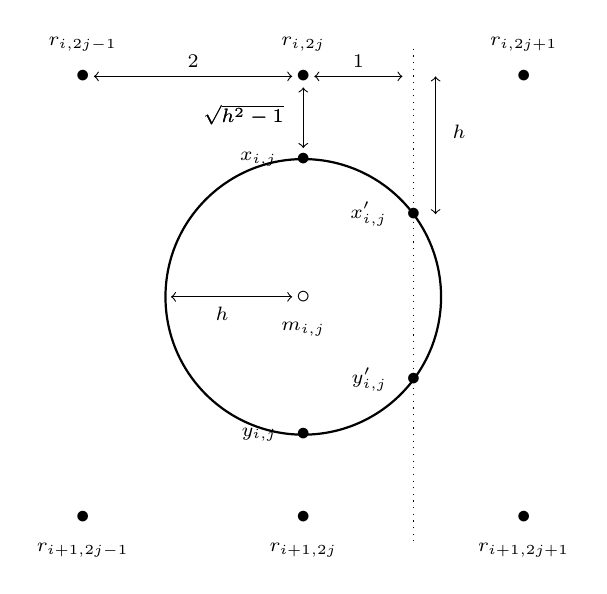
\begin{tikzpicture}[scale=7]

	
	\node[label=90:\scriptsize $r_{i,2j-1}$] at (0.1,0) {$\bullet$};
	\node[label=90:\scriptsize $r_{i,2j}$] at (0.5,0) {$\bullet$};
	\node[label=90:\scriptsize $r_{i,2j+1}$] at (0.9,0) {$\bullet$};
	
	\node[label=180:\scriptsize $\sqrt{h^2-1}$] at (0.5,-0.07) {};
	\node[label=180:\scriptsize $x_{i,j}$] at (0.5,-0.15) {$\bullet$};
	
	
	\node[label=180:\scriptsize $h$] at (0.83,-0.1) {};
	\node[label=180:\scriptsize $x_{i,j}'$] at (0.7,-0.25) {$\bullet$};
	
	\node[label=270:\scriptsize $m_{i,j}$] at (0.5,-0.4) {$\circ$};
	
	
	\node[label=180:\scriptsize $y_{i,j}$] at (0.5,-0.65) {$\bullet$};
	\node[label=180:\scriptsize $y_{i,j}'$] at (0.7,-0.55) {$\bullet$};
	
	
	\node[label=270:\scriptsize $r_{i+1,2j-1}$] at (0.1,-0.8) {$\bullet$};
	\node[label=270:\scriptsize $r_{i+1,2j}$] at (0.5,-0.8) {$\bullet$};
	\node[label=270:\scriptsize $r_{i+1,2j+1}$] at (0.9,-0.8) {$\bullet$};
	
	
	\node[label=180:\scriptsize $\sqrt{h^2-1}$] at (0.5,-0.07) {};
	
	
	\node[label=180:\scriptsize $h$] at (0.4,-0.43) {};
	\node[label=90:\scriptsize $1$] at (0.6,-0.02) {};
	\node[label=90:\scriptsize $2$] at (0.3,-0.02) {};
	
	
	\draw[<->] (0.5,-0.13) -- (0.5,-0.02);
	\draw[<->] (0.26,-0.4) -- (0.48,-0.4);
	\draw[dotted,-] (0.7, 0.05) -- (0.7, -0.85);
	\draw[<->] (0.74, 0.0) -- (0.74, -0.25);
	\draw[<->] (0.68, 0.0) -- (0.52, 0.0);
	\draw[<->] (0.12, 0.0) -- (0.48, 0.0);
	\draw[black, thick] (0.5,-0.4) circle (0.25);
\end{tikzpicture}


\ifdefined\COMPLETE
\else
\end{document}
\fi

    \caption{The locations of $x_{i,j}$, $x_{i,j}'$, $y_{i,j}$ and $y_{i,j}'$ in the set $Z_i$. The points in bullet have weight $w$ while the points in circles have weight $2w$.}
    \label{fig:ZFig}
  \end{minipage}
\end{figure}
  




\subsubsection{Properties of the Construction}

In this section we show some properties of the construction that will ultimately enable us to prove Theorem \ref{thm:gammaLower}. These definitions will be useful throughout the section

$$L_1 = (6m+3)wl, L_2 = 3m(l-1)w, L=L_1 + L_2 -m\alpha, \alpha = \frac{d}{w}-\frac{1}{2w^3}$$

\begin{definition}[$A$- and $B$-Clustering of $R_i$]
\label{defn:abclusteringVattani}

An $A$-Clustering of row $R_i$ is a clustering in the form of $\{\{s_i\}, \{r_{i,1}, r_{i,2}\}, \{r_{i,3}, r_{i,4}\}, \ldots, \{r_{i,6m-1}, r_{i,6m}\},\{r_{i, 6m+1}, f_i\}\}$. A $B$-Clustering of row $R_i$ is a clustering in the form of $\{\{s_i, r_{i, 1}\}, \{r_{i,2}, r_{i,3}\}, \{r_{i,4}, r_{i,5}\}, \ldots, \{r_{i,6m}, r_{i,6m+1}\},\{f_i\}\}$. 
\end{definition}

\begin{definition}[Good point for a cluster]
\label{defn:goodPointVattani}
A cluster $C$ is good for a point $z \not\in C$ if adding $z$ to $C$ increases cost by exactly $\frac{2w}{3}h^2$ 
\end{definition}

Given the above definition, the following simple observations can be made. 
\begin{itemize}[nolistsep,noitemsep]
\item The clusters $\{r_{i,2j-1}, r_{i, 2j}\}$, $\{r_{i,2j}, r_{i, 2j+1}\}$ and $\{g_{i,j}\}$ are good for $x_{i,j}$ and $y_{i-1,j}$.
\item The clusters $\{r_{i,2j}, r_{i, 2j+1}\}$ and $\{g_{i,j}\}$ are good for $x_{i,j}'$ and $y_{i-1,j}'$.
\end{itemize}

\begin{definition}[Nice Clustering]
\label{defn:niceClustering}
A $k$-clusteirng is nice if every $g_{i,j}$ is a singleton cluster, each $R_i$ is grouped in the form of either an $A$-clustering or a $B$-clustering and the points in $Z_i$ are added to a cluster which is good for it.
\end{definition}

It is straightforward to see that a row grouped in a $A$-clustering costs $(6m+3)w-\alpha$ while a row in $B$-clustering costs $(6m+3)w$. Hence, a nice clustering of $H_{l,m} \cup Z$ costs at most $L_1 + L_2$. More specifically, if $t$ rows are group in a $A$-clustering, the nice-clustering costs $L_1+L_2-t\alpha$. Also, observe that any nice clustering of $X$ has only the following four different types of clusters. \begin{enumerate}[label=(\arabic*),nolistsep,leftmargin=*]
\item Type E - $\{r_{i,2j-1}, r_{i,2j+1}\}$ \\
The cost of this cluster is $2w$ and we define the contribution of each location as  cost/no. of locations $ = \frac{2w}{2} = w$.
\item Type F - $\{r_{i,2j-1}, r_{i, 2j}, x_{i, j}\}$ or $\{r_{i,2j-1}, r_{i, 2j}, y_{i-1, j}\}$ or $\{r_{i,2j}, r_{i, 2j+1}, x_{i, j}'\}$ or $\{r_{i,2j}, r_{i, 2j+1}, y_{i-1, j}'\}$\\
The cost of any cluster of this type is $2w(1+\frac{h^2}{3})$ and the contribution of each location to is atmost $\frac{2w}{9}(h^2+3)$. For $h = \sqrt 5$, this equals $\frac{16}{9}w$.  
\item Type I - $\{g_{i, j}, x_{i,j}\}$ or $\{g_{i, j}, x_{i,j}'\}$  or $\{g_{i, j}, y_{i,j}\}$  or $\{g_{i, j}, y_{i,j}'\}$\\
The cost of any cluster of this type is $\frac{2}{3}wh^2$ and the contribution to cost of each location is $\frac{w}{3}h^2$. For our choice of $h$, the contribution is $\frac{5}{3}w$.
\item Type J - $\{s_i, r_{i,1}\}$ or $\{r_{i,6m+1}, f_i\}$\\
The cost of this cluster is $3w$ (or $3w-\alpha$) and we define the contribution of each location to cost is atmost $1.5w$. 
\end{enumerate}
Hence, observe that in a nice-clustering, any location contributes atmost $\le \frac{16}{9}w$ to the total clustering cost. This observation will be useful in the proof of the lemma below.

\begin{lemma}
\label{lemma:costNonNice}
For large enough $w = poly(l, m)$, any non-nice clustering of $X = H_{l, m} \cup Z$ costs at least $L + cw$ for any $c < \frac{1}{3}$.
\end{lemma}

\begin{proof}
We will show that any non-nice clustering $C$ of $X$ costs atleast $w$ more than the cost of any nice clustering. This will prove our result. The following cases are possible.

\begin{itemize}[nolistsep,leftmargin=*]
\item $C$ contains a cluster $C_i$ of cardinality $t > 6$\\
Observe that any $x \in C_i$ has at least $t-5$ locations at a distance $\ge 4$ and $4$ locations at a distance atleast $2$. Hence, the cost of $C_i$ is atleast $\frac{w}{2t}(4^2(t-5)+2^24)t = 8w(t-4)$. $C_i$ allows us to use atmost $t-2$ singletons. This is because a nice clustering of these $t+(t-2)$ points uses atmost $t-1$ clusters and the clustering $C$ uses  $1 + (t-2)$ clusters for these points. The cost of the nice cluster on these points is $\le \frac{16w}{9}2(t-1)$. While the non-nice clustering costs atleast $8w(t-4)$. For $t \ge 6.4 \implies 8(t-4) > \frac{32}{9}(t-1)$ and the claim follows. Note that in this case the difference in cost is atleast $\frac{8w}{3}$. 

\item Contains a cluster of cardinality $t = 6$\\
Simple arguments show that amongst all clusters of cardinality $6$, the following has the minimum cost. $C_i = \{r_{i, 2j-1}, r_{i, 2j}, x_{i,j}, y_{i-1, j}, r_{i, 2j+1}, r_{2j+2}\}$. The cost of this cluster is $\frac{176w}{6}$. Arguing as before, this allows us to use $4$ singletons. Hence, a nice cluster on these $10$ points costs atmost $\frac{160w}{9}$. The difference of cost is atleast $34w$.  

\item Contains a cluster of cardinality $t = 5$\\
Simple arguments show that amongst all clusters of cardinality $5$, the following has the minimum cost. $C_i = \{r_{i, 2j-1}, r_{i, 2j}, x_{i,j}, y_{i-1, j}, r_{i, 2j+1}\}$. The cost of this cluster is $16w$. Arguing as before, this allows us to use $3$ singletons. Hence, a nice cluster on these $8$ points costs atmost $16w\frac{8}{9}$. The difference of cost is atleast $\frac{16w}{9}$.  

\item Contains a cluster of cardinality $t = 4$\\
It is easy to see that amongst all clusters of cardinality $4$, the following has the minimum cost. $C_i = \{r_{i, 2j-1}, r_{i, 2j}, x_{i,j}, r_{i, 2j+1}\}$. The cost of this cluster is $11w$. Arguing as before, this allows us to use $2$ singletons. Hence, a nice cluster on these $6$ points costs atmost $\frac{32w}{3}$. The difference of cost is atleast $\frac{w}{3}$.

\item All the clusters have cardinality $\le 3$ \\
Observe that amongst all non-nice clusters of cardinality $3$, the following has the minimum cost. $C_i = \{r_{i, 2j-1}, r_{i, 2j}, r_{i, 2j+1}\}$. The cost of this cluster is $8w$. Arguing as before, this allows us to use atmost $1$ more singleton. Hence, a nice cluster on these $4$ points costs atmost $\frac{64w}{9}$. The difference of cost is atleast $\frac{8w}{9}$.

It is also simple to see that any non-nice clustering of size $2$ causes an increase in cost of atleast $w$.

\end{itemize}
\end{proof}

\begin{lemma}
\label{lemma:kmeansEquivalenceX3C}
The set $X = H_{l,n} \cup Z$ has a $k$-clustering of cost less or equal to $L$ if and only if there is an exact cover for the X3C instance.
\end{lemma}
\begin{proof}
The proof is identical to the proof of Lemma 11 in \cite{vattani2009hardness}. Lemma 11 in Vattani's paper uses Lemma 10 to argue why the only nice clusterings of $X$ cost $\le L$. We use Lemma \ref{lemma:costNonNice} to argue the same. Note that since the parameters are much different that those considered in Vattani's original construction, we need to argue much more carefully to prove Lemma \ref{lemma:costNonNice}. 
\end{proof}

\begin{lemma}
\label{lemma:gammaLower}
Any clustering of $X = H_{l,n} \cup Z$ which has cost$\le L$ has the $\gamma$-margin property where $\gamma = \sqrt{\frac{17}{5}} \approx 1.84$.
\end{lemma}
\begin{proof}
As argued before, any nice clustering has four different types of clusters. We will calculate the minimum ratio $a_i = \frac{d(y, \mu)}{d(x, \mu)}$ for each of these clusters $C_i$ (where $x \in C_i$, $y \not\in C_i$ and $\mu$ is mean of all the points in $C_i$.) Then, the minimum $a_i$ will give the desired $\gamma$. 
\begin{enumerate}[label=(\arabic*),nolistsep,leftmargin=*]
\item For Type E clusters $a_i = h/1 = \sqrt{5}$. 
\item For Type F clusters. $a_i = \frac{\frac{\sqrt{4+16(h^2-1)}}{3}}{2h/3} = \sqrt{\frac{17}{5}} \approx 1.84$. 
\item For Type I clusters, standard calculation show that $a_i > 2$.
\item For Type J clusters $a_i = \frac{2+\frac{\sqrt{6}}{2}}{\frac{\sqrt{6}}{2}} > 2$.
\end{enumerate}
\end{proof}
Lemmas \ref{lemma:kmeansEquivalenceX3C} and \ref{lemma:gammaLower} complete the proof of the main result (Thm. \ref{thm:gammaLower}). 

\section{Concentration inequalities}
\label{appendixsection:conIneq}

\begin{theorem}[Generalized Hoeffding's Inequality (e.g., \cite{ashtiani2015dimension})]
\label{thm:genHoeff}
Let $X_1, \ldots. X_n$ be i.i.d random vectors in some Hilbert space such that for all $i$, $\|X_i\|_2 \le R$ and $E[X_i] = \mu$. If $n > c\frac{\log(1/\delta)}{\epsilon^2}$, then with probability atleast $1-\delta$, we have that
$$\Big\|\mu - \frac{1}{n}\sum X_i\Big\|_2^2 \le R^2\epsilon$$ 
\end{theorem}


%\section{Concentration inequalities}
%\label{appendixsection:proofs}

%It is easy to see that in the optimal solution of $k$-means objective function, $\mu_i$ is the center of mass of $C_i$, i.e., $\mu_i = \frac{1}{|C_i|}\sum_{x\in C_i}x$. Also, the objective function can be rewritten in the following form (E.g., see \cite{inaba1994applications})

%$$f(\mc C) = \sum\limits_{C_i}\frac{1}{|C_i|} \sum_{x, y \in C_i} d^2(x, y).$$

\bibliographystyle{alpha}
\bibliography{activeClustering}
\end{document}


